\graphicspath{{images/}}

\section{Lineare Abbildungen}


\begin{definition}{Lineare Abbildung} $f: V \rightarrow W$ wo $V$, $W$ reelle Vektorräume\\
    Eine Abbildung $f$ heisst linear, wenn $\forall \overrightarrow{a}, \overrightarrow{b} \in V$, $\forall \lambda \in \mathbb{R}$ gilt:
    $$
    f(\overrightarrow{a} + \overrightarrow{b}) = f(\overrightarrow{a}) + f(\overrightarrow{b})
    \text{ und }
    f(\lambda \cdot \overrightarrow{a} \cdot \vec{b}) = \lambda \cdot f(\overrightarrow{a}) \cdot f(\vec{b})
    $$
    Erlaubte Operationen:\\
    \begin{minipage}{0.6\linewidth}
        \begin{itemize}
            \item Multiplikation mit Skalar: $\lambda \cdot \vec{a}$
        \end{itemize}
    \end{minipage}
    \begin{minipage}{0.3\linewidth}
        \begin{itemize}
            \item Addition: $\vec{a} + \vec{b}$
        \end{itemize}
    \end{minipage}
    
    \vspace{1mm}

    Verbotene Operationen:\\
    \begin{minipage}{0.6\linewidth}
        \begin{itemize}
            \item Multiplikation von Vektoren: $\vec{a} \cdot \vec{b}$
            \item Addition von Skalaren: $\lambda + \vec{a}$
        \end{itemize}
    \end{minipage}
    \begin{minipage}{0.3\linewidth}
        \begin{itemize}
            \item Potenzieren: $\vec{a}^2$
            \item Cosinus: $\cos(\vec{a})$
        \end{itemize}
    \end{minipage}
\end{definition}

\begin{KR}{Überprüfung der Linearität}
    $f: V \rightarrow W$, $f(\vec{x}) \rightarrow \vec{y}$
    \begin{itemize}
        \item $f(\vec{0}) = \vec{0}$
        \item $f(\lambda \cdot \overrightarrow{x_1} \cdot \vec{x_2}) = \lambda \cdot f(\overrightarrow{a}) \cdot f(\vec{b})$
        \item $f(\vec{x_1} + \vec{x_2}) = f(\vec{x_1}) + f(\vec{x_2})$
    \end{itemize}

    \vspace{1mm}

    $\Rightarrow$ Funktionsgleichung einsetzen und überprüfen
\end{KR}

\begin{example}
    $f: \mathbb{R} \rightarrow \mathbb{R}: f(x)=\binom{x_{1}}{x_{2}} \rightarrow\binom{x_{1}+2 x_{2}}{x_{2}}$
    $$
    f\binom{x_{1}+y_{1}}{x_{2}+y_{2}}=\binom{x_{1}+y_{1}+2 \cdot\left(x_{2}+y_{2}\right)}{x_{2}+y_{2}}
    =f\binom{x_{1}}{x_{2}}+f\binom{y_{1}}{y_{2}} \Rightarrow \surd 
    $$
    ... usw.
\end{example}


\begin{definition}{Bild im(A)}
    einer $m \times n$-Matrix $A$, ist der Unterraum des m-dimensionalen Vektorraum $W$, der von den Spalten $\overrightarrow{a_{1}}, \overrightarrow{a_{2}}, \ldots, \overrightarrow{a_{n}}$ der Matrix aufgespannt wird:
    $$
    \operatorname{im}(A)=\operatorname{span}\left(\overrightarrow{a_{1}}, \ldots, \overrightarrow{a_{n}}\right)=\left\{\lambda_{1} \overrightarrow{a_{1}}+\cdots+\lambda_{n} \overrightarrow{a_{n}} \mid \lambda_{1} \in \mathbb{R}\right\}
    $$
\end{definition}

\begin{definition}{Kern ker(A)}
    einer $m \times n$-Matrix $A$ ist die Lösungsmenge des homogenen LGS $A \cdot \vec{x}=\overrightarrow{0}$. Der Kern $\operatorname{ker}(A)$ ist der folgende Unterraum von $V$
    $$\operatorname{ker}(A)=\{\vec{x} \in V \mid A \cdot \vec{x}=\overrightarrow{0}\}$$
\end{definition}



\begin{KR}{Basis für Bild und Kern}
    1. Bringe $A$ in Zeilenstufenform (ZSF)

    \vspace{1mm}

    \begin{minipage}{0.45\linewidth}
        \textcolor{pink}{Bild:}\\
        2. Pivotspalten in der ZSF?\\
        3. Pivotspalten von $A$ (nicht ZSF!) ergeben eine Basis für den Kern
    \end{minipage}
    \hspace{3mm}
    \begin{minipage}{0.5\linewidth}
        \textcolor{pink}{Kern:}\\
        2. LGS $A \cdot \vec{x} = \overrightarrow{0}$ aufstellen\\
        3. Lösungsmenge als LK von Vektoren mit freien Variablen als Koeffizienten ergibt Basis für Kern
    \end{minipage}
\end{KR}



\begin{example}
    \resizebox{\textwidth}{!}{
    $ A = \begin{pmatrix} -1 & 0 & 2 \\ 1 & 6 & 4 \\ 3 & 3 & -3 \end{pmatrix} 
    \Rightarrow \left(\begin{array}{ccc|c}
        -1 & 0 & 2 & 0 \\
        1 & 6 & 4 & 0 \\
        3 & 3 & -3 & 0
        \end{array}\right)=\left(\begin{array}{ccc|c}
        1 & 0 & -2 & 0 \\
        0 & 1 & 1 & 0 \\
        0 & 0 & 0 & 0
        \end{array}\right)
    $}

    \vspace{1mm}

    $$
    x_{1}=2 \lambda, x_{2}=-\lambda, x_{3}=\lambda
    $$

    \vspace{2mm}

    \resizebox{\textwidth}{!}{
    $
    im(A) = \left\{\begin{psmallmatrix} -1 \\ 1 \\ 3 \end{psmallmatrix} \cdot \mu + \begin{psmallmatrix} 0 \\ 6 \\ 3 \end{psmallmatrix} \cdot v \mid \mu, v \in \mathbb{R}\right\}
    \quad
    ker(A) = \left\{\begin{psmallmatrix} 2 \\ -1 \\ 1 \end{psmallmatrix} \cdot \lambda \mid \lambda \in \mathbb{R}\right\}
    $}
\end{example}



\begin{formula}{Zauberzahlen m{,} n{,} r{,}} Für $A^{m \times n}$ mit $rg{A} = r$ gilt:
    $$
    \dim(im(A))=\dim(im(A^{-1}))=r
    $$
    $$
    \dim(ker(A))=n-r
    \text{ und } \dim(ker(A^{-1}))=m-r
    $$
\end{formula}

\subsubsection*{Abbildungsmatrix}

\begin{definition}{Homogene Koordinaten}
    Homogene Koordinaten sind eine Erweiterung des euklidischen Raumes, die es ermöglicht, Punkte im Unendlichen zu repräsentieren.
    Ein Punkt im $\mathbb{R}^2$ wird durch einen Vektor $(x, y, z)$ dargestellt, wobei $z\neq 0$.
    Die Punkte $(x, y, z)$ und $(\lambda x, \lambda y, \lambda z)$ repräsentieren den gleichen Punkt im euklidischen Raum.
    
    {\small nützlich, um Transformationen wie Translationen und Projektionen zu vereinfachen}
\end{definition}

\begin{definition}{Abbildungsmatrix STandardbasis}
    Vektorräume $\mathbb{R}^{m}$ und $\mathbb{R}^{n}$, mit der jeweiligen Standardbasis. Dann lässt sich jede lineare Abbildung $f: \mathbb{R}^{n} \rightarrow \mathbb{R}^{m}$ durch eine $m \times n$ - Matrix $A$ darstellen

    $$
    f(\vec{x})=A \cdot \vec{x}
    $$

    Die Spalten der Matrix $A$ sind die Bilder der Standardbasisvektoren von $\mathbb{R}^{n}$ :

    \begin{center}
    \resizebox{0.7\textwidth}{!}{
    $
    A = \left(f(\overrightarrow{e_{1}}) \scalebox{0.5}{\ldots} f(\overrightarrow{e_{n}})\right)
    = \left(f\begin{psmallmatrix} 1 \\ 0 \\ \scalebox{0.5}{\vdots} \\ 0 \end{psmallmatrix} f\begin{psmallmatrix} 0 \\ 1 \\ \scalebox{0.5}{\vdots} \\ 0 \end{psmallmatrix} \scalebox{0.5}{\ldots} f\begin{psmallmatrix} 0 \\ 0 \\ \scalebox{0.5}{\vdots} \\ 1 \end{psmallmatrix}\right)
    $}
    \end{center}
\end{definition}

\begin{example}
    $$
    f: \mathbb{R}^{2} \rightarrow \mathbb{R}^{3}:\binom{x_{1}}{x_{2}} \rightarrow \begin{psmallmatrix} x_{1}-x_{2} \\ 3 x_{2} \\ -4 x_{1} \end{psmallmatrix}
    \Rightarrow A = \begin{psmallmatrix} 1 & -1 \\ 0 & 3 \\ -4 & 0 \end{psmallmatrix}
    $$
\end{example}

\begin{formula}{Abbildungsmatrix beliebiger Basis}\\
    Wir betrachten zwei endliche Vektorräume
    $$
    V \text { mit Basis } B=\left\{\overrightarrow{b_{1}} ; \ldots ; \overrightarrow{b_{n}}\right\}, W \text { mit Basis } C=\left\{\overrightarrow{c_{1}} ; \ldots ; \overrightarrow{c_{n}}\right\}
    $$

    Jede lineare Abbildung $f: V \rightarrow W$ lässt sich durch eine $m \times n$ - Matrix ${ }_{C} A_{B}$ darstellen

    $$
    (f(\vec{x}))_{C}={ }_{C} A_{B} \cdot \vec{x}_{B}
    $$

    Die Spalten der Matrix ${ }_{C} A_{B}$ sind die Bilder der Elemente von $B$ in der Komponentendarstellung bezüglich der Basis $C$ :
    \begin{center}
    \resizebox{0.8\textwidth}{!}{
    $
    { }_{C} A_{B}={ }_{C}\left(\left(f\left(\overrightarrow{b_{1}}\right)\right)_{C}\left(f\left(\overrightarrow{b_{2}}\right)\right)_{C} \quad \cdots \quad\left(f\left(\overrightarrow{b_{n}}\right)\right)_{C}\right)_{B}
    $
    }
    \end{center}
\end{formula}

\begin{example}
    $$
    f: \mathbb{R}^{2} \rightarrow \mathbb{R}^{3}:\binom{x_{1}}{x_{2}} \rightarrow\begin{psmallmatrix} x_{1}-x_{2} \\ 3 x_{2} \\ -4 x_{1} \end{psmallmatrix}
    $$

    $$
    B=\left\{\binom{1}{0} ; \binom{0}{1}\right\}, C=\left\{\binom{1}{0} ; \binom{1}{1} ; \binom{1}{2}\right\}
    \Rightarrow { }_{C} A_{B}=\begin{psmallmatrix} 1 & -1 \\ 0 & 3 \\ -4 & 0 \end{psmallmatrix}
    $$
\end{example}



\begin{theorem}{Verknüpfungen}
    Wir betrachten zwei lineare Abbildungen
    \begin{itemize}
    \item $f: U \rightarrow V$ mit Abbildungsmatrix $A$
    \item $g: V \rightarrow W$ mit Abbildungsmatrix $B$
    \end{itemize}
    \begin{center}
    \includegraphics[width=0.4\textwidth]{verknüpfungen.png}\\
    \end{center}
    Die Abbildungsmatrix der Verknüpfung $g \circ f$ ist wieder eine lineare Abbildung mit der Abbildungsmatrix $B \cdot A$.
\end{theorem}

\begin{concept}{Koordinatentransformation}\\
    Die Abbildungsmatrix ${ }_{B} T_{S}$ für den Basiswechsel von $S$ nach $B$
    \begin{itemize}
    \item Die Matrix ${ }_{B} T_{S}$ ist die Inverse von ${ }_{S} T_{B}:{ }_{B} T_{S}=\left({ }_{S} T_{B}\right)^{-1}$
    \end{itemize}
    \begin{center}
    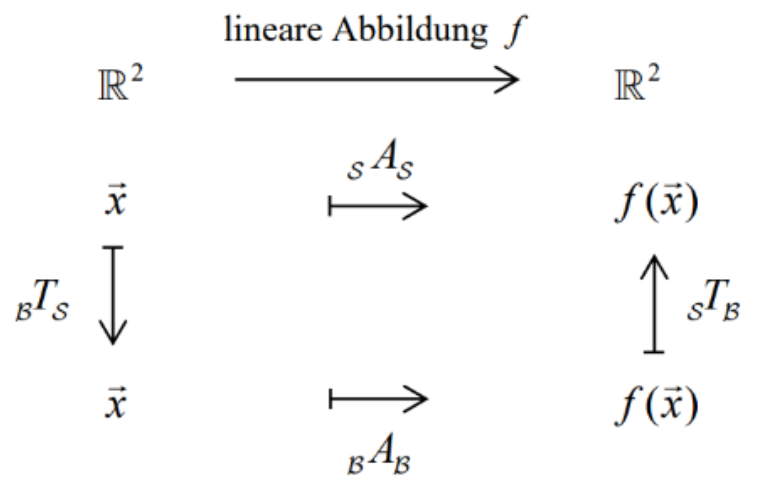
\includegraphics[width=0.6\textwidth]{koordinatentransformation.png}
    \end{center}
\end{concept}

\begin{KR}{Basiswechsel mit Koordinatentransformation}\\
    \begin{minipage}{0.45\linewidth}
        \textcolor{pink}{Von Basis $B$ nach Basis $C$}
        $$
        \vec{x}_{C}={ }_{C} T_{B} \cdot \vec{x}_{B}
        $$
        ${ }_{C} T_{B} :=$ Abbildungsmatrix\\ von $B$ nach $C$
        $${ }_{C} T_{B} = { }_{C} A_{S} \cdot { }_{S} T_{B}$$
    \end{minipage}
    \hspace{3mm}
    \begin{minipage}{0.45\linewidth}
        \textcolor{pink}{Von Basis $C$ nach Basis $B$}
        $$
        \vec{x}_{B}={ }_{B} T_{C} \cdot \vec{x}_{C}
        $$
        ${ }_{B} T_{C} :=$ Abbildungsmatrix\\ von $C$ nach $B$
        $${ }_{B} T_{C} = { }_{B} A_{S} \cdot { }_{S} T_{C}$$
    \end{minipage}
\end{KR}

\begin{example}
    $$
    B=\left\{\binom{2}{5}_{S} ;\binom{-1}{3}_{S}\right\}, \quad C=\left\{\binom{1}{0}_{S} ;\binom{1}{1}_{S} ;\binom{1}{2}_{S}\right\}
    $$
    $$
    { }_{C} T_{B}=\left(\begin{array}{cc}
    2 & -1 \\
    5 & 3
    \end{array}\right), \quad { }_{B} T_{C}=\left({ }_{C} T_{B}\right)^{-1}=\left(\begin{array}{cc}
    3 & 1 \\
    -5 & 2
    \end{array}\right)
    $$
\end{example}

\begin{KR}{Vollständiges Beispiel} 
    \\Kann mittels Inverse oder Gauss berechnet werden

    $$
    f: \mathbb{R}^{2} \rightarrow \mathbb{R}^{3}:\binom{x_{1}}{x_{2}} \rightarrow\begin{psmallmatrix} -x_{2} \\ 2 x_{1} \\ x_{2}-x_{1} \end{psmallmatrix}
    $$

    $$
    B=\left\{\binom{2}{5}_{S} ;\binom{-1}{3}_{S}\right\}, C=\left\{\begin{psmallmatrix} 1 \\ 0 \\ 1 \end{psmallmatrix}_{S} ;\begin{psmallmatrix} 0 \\ 2 \\ 1 \end{psmallmatrix}_{S} ;\begin{psmallmatrix} 1 \\ -4 \\ 1 \end{psmallmatrix}_{S}\right\}
    $$

    $$
    { }_{C} A_{B}={ }_{C}\left(\left(f\left(\frac{2}{5}\right)\right)_{C}\left(f\binom{-1}{3}\right)_{C}\right)_{B}
    $$

    \vspace{2mm}

    \resizebox{\textwidth}{!}{
    $
    \left(f \binom{2}{5}\right)_{C}=\begin{psmallmatrix} -5 \\ 4 \\ 3 \end{psmallmatrix}_{C}
    = \left(\begin{array}{ccc|c}
        1 & 0 & 1 & -5 \\
        0 & 2 & -4 & 4 \\
        1 & 1 & 1 & 3
        \end{array}\right)=\left(\begin{array}{ccc|c}
        1 & 0 & 0 & -11 \\
        0 & 1 & 0 & 14 \\
        0 & 0 & 1 & 6
        \end{array}\right)
    $}

    \vspace{2mm}

    \resizebox{\textwidth}{!}{
    $
    \left(f \binom{-1}{3}\right)_{C}=\begin{psmallmatrix} -3 \\ -2 \\ 4 \end{psmallmatrix}_{C}
    = \left(\begin{array}{ccc|c}
        1 & 0 & 1 & -3 \\
        0 & 2 & -4 & -2 \\
        1 & 1 & 1 & 4
        \end{array}\right)=\left(\begin{array}{ccc|c}
        1 & 0 & 0 & -11 \\
        0 & 1 & 0 & 15 \\
        0 & 0 & 1 & 8
        \end{array}\right)
    $}
    \vspace{2mm}
    
    $$
    { }_{C} A_{B}=\begin{psmallmatrix} -11 & -11 \\ 14 & 15 \\ 6 & 8 \end{psmallmatrix}_{B}
    $$
\end{KR}
